\documentclass[11pt,oneside]{article}
\input{../../../Header/packages.sty}
\input{../../../Header/styleScript.sty}
\input{../../../Header/headerScript.sty}
\input{../../../Header/mathexpressions.sty}
\graphicspath{{images/}}

\newcommand{\Skriptname}{Geometrie  Einführung}
\newcommand{\Autor}{Jonas Guler (Gu)}

\begin{document}   % KSH-Guler - OneNote oder Atchu -> PDF/Latex
\begin{titlepage}
	\clearpage
	\title{\Huge\textbf{\Skriptname} \\[1cm]}
	\author{Autor:\\ \Autor}
	\date{\normalsize {Version 1.1}\\ \datelong}
	\maketitle
	\thispagestyle{empty}
	\vfill
	\tableofcontents
\end{titlepage}
\pagenumbering{arabic}
%############################################################################################
\section{Begriffe, Winkel an Geraden}
	\vspace{5pt}
	\begin{definition}
		\begin{minipage}{0.6\linewidth}
			Zwei Strahlen mit gemeinsamen Anfangspunkt $S$ bilden einen \textbf{Winkel}. $S$ ist der \textbf{Scheitel} des Winkels, die beiden Strahlen werden als \textbf{Schenkel} bezeichnet.\vspace{11pt}\newline
			Kennt man zwei Punkte auf je einem Schenkel, so wird der Winkel mit $\angle ASB$.
		\end{minipage}
		\hfill
		\begin{minipage}{0.35\linewidth}
			\centering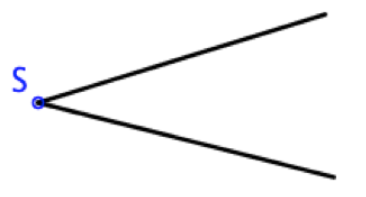
\includegraphics[scale=0.4]{Def-Winkel.png}
		\end{minipage}
	\end{definition}
	\begin{notation}
		Winkel werden mit den griechischen Kleinbuchstaben bezeichnet.
		\begin{enumerate}[label=\ ]\begin{multicols}{3}
				\item $\alpha\quad$ Alpha
				\item $\beta\quad$ Beta
				\item $\gamma\quad$ Gamma
				\item $\delta\quad$ Delta
				\item $\epsilon\quad$ Epsilon
				\item $\ldots$
		\end{multicols}\end{enumerate}
	\end{notation}
	Die Grösse eines Winkel kann mithilfe des Geodreiecks bestimmt werden. Dabei bezeichnen wir unterschiedlich grosse Winkel wie folgt:
	\begin{table}[H]
		\centering
		\begin{tabular}{m{4cm} m{4cm} m{7cm}}
			spitzer Winkel & 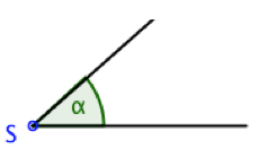
\includegraphics[width=3cm]{spitzerWinkel.png} & wenn $\alpha$ zwischen $0^\circ$ und $90^\circ$\\
			rechter Winkel & 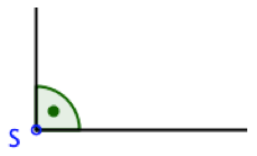
\includegraphics[width=3cm]{rechterWinkel.png} & wenn $\alpha=90^\circ$\\
			stumpfer Winkel & 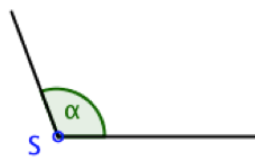
\includegraphics[width=3cm]{stumpferWinkel.png} & wenn $\alpha$ zwischen $90^\circ$ und $180^\circ$\\
			gestreckter Winkel & 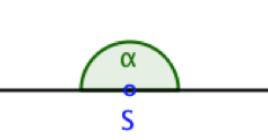
\includegraphics[width=3cm]{gestreckterWinkel.png} & wenn $\alpha=180^\circ$\\
			überstumpfer Winkel & 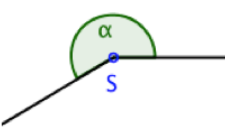
\includegraphics[width=3cm]{überstumpferWinnkel.png} & wenn $\alpha$ zwischen $180^\circ$ und $360^\circ$\\
		\end{tabular}
	\end{table}
	Falls wir mehrere Winkel miteinander vergleichen möchten, können wir für zwei sich schneidende Geraden folgenden Satz formulieren.
	\begin{satz}[Neben- und Scheitelwinkel]
		\begin{minipage}{0.6\linewidth}
			Winkel, die sich bei einer Geradenkreuzung nebeneinander befinden, heissen \textbf{Nebenwinkel}. Winkel, die sich bei einer Geradenkreuzung gegenüber befinden, heissen \textbf{Scheitelwinkel}. Für diese beiden Winkel gelten folgende Aussagen:
			\begin{enumerate}
				\item Die Summe zweier Nebenwinkel beträgt $180^\circ$.
				\item Scheitelwinkel sind gleich gross.
			\end{enumerate}
		\end{minipage}
		\hfill
		\begin{minipage}{0.35\linewidth}
			\centering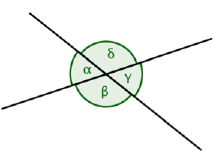
\includegraphics[scale=0.7]{scheitelwinkel.png}
		\end{minipage}
	\end{satz}
	Auf der anderen Seite können wir für zwei parallele Geraden ebenfalls einen Satz formulieren.
	\begin{satz}[Stufen- und Wechselwinkel]
		Für \textbf{Stufen-} und \textbf{Wechselwinkel}, die in der untenstehenden Grafik veranschaulicht werden, gilt folgende Aussage:
		\begin{center}
			\begin{figure}[H]
				\centering
				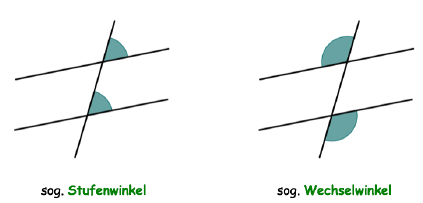
\includegraphics[scale=0.7]{stufenwinkel.png}
			\end{figure}
			Stufen- und Wechselwinkel sind gleich gross.
		\end{center}
	\end{satz}\newpage


\section{Winkelsätze bei Figuren}
	Vermutlich kennt ihr alle bereits die Winkelsumme eines Dreiecks. Jedoch habt ihr die Aussage wohl kaum riguros bewiesen. Da das Beweisen auch als Königsdisziplin der Mathematik betrachtet wird, möchte ich diese Aussage beispielhaft beweisen.
	\begin{satz}[Winkelsumme im Dreieck]
		In jedem Dreieck gilt: $\alpha+\beta+\gamma=180^\circ$.
	\end{satz}
	\begin{beweis}
		\karos{3.5}
	\end{beweis}
	Lasst uns die Winkelsumme für ein beliebiges Vieleck untersuchen.
	\begin{aufgabe}
		\begin{enumerate}[label=\alph*)]
			\item Dazu starten wir bei einem Viereck und zerlegen dieses in zwei Dreiecke, indem wir eine Diagonale einzeichnen. Zeichne eine Skizze und gib die Winkelsumme eines Vierecks an.
		\end{enumerate}
		\karos{4}
		\begin{enumerate}[label=\alph*)]\setcounter{enumi}{1}
			\item Und im Fünfeck? Zeichne auch hier verschiedene Möglichkeiten, um das Fünfeck in Dreiecke zu unterteilen und berechne die Winkelsumme.
		\end{enumerate}
		\karos{4}
		\begin{enumerate}[label=\alph*)]\setcounter{enumi}{2}
			\item Und im Siebeneck? Zeichne auch hier verschiedene Möglichkeiten, um das Siebeneck in Dreiecke zu unterteilen und berechne die Winkelsumme.
		\end{enumerate}
		\karos{4}
		\begin{enumerate}[label=\alph*)]\setcounter{enumi}{3}
			\item Zusammenfassend stelle eine Formel auf, die die Winkelsumme eines Vielecks in Abhängigkeit der Anzahl Eckpunkten $n$ berechnet.
		\end{enumerate}
		\karos{2}
	\end{aufgabe}
	\begin{satz}[Winkelsumme im $n-$Eck]
		Die Winkelsumme eines $n-$Eck lässt sich mit der folgenden Formel berechnen:\[\gap{5}.\]
	\end{satz}
	\begin{aufgabe}
		Löse die Aufgaben zur Winkelberechnungen.
	\end{aufgabe}

\subsection{Der Satz des Thales}
	\begin{minipage}{0.6\linewidth}
		Wir betrachten einen Halbkreis mit gegebenem Durchmesser $\overline{AB}$. Irgendwo auf dem Halbkreis wählen wir einen weiteren Punkt $C$.\vspace{11pt}\newline
		Da $\overline{AM}=\overline{BM}=\overline{CM}$ (Radius des Halbkreis), sind die Dreiecke $\triangle AMC$ und $\triangle BMC$ gleichschenklig und haben also jeweils zwei gleich grosse Winkel.
	\end{minipage}
	\hfill
	\begin{minipage}{0.35\linewidth}
		\centering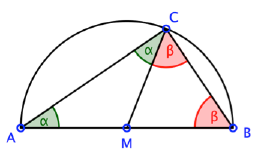
\includegraphics[scale=0.7]{thaleskreis.png}
	\end{minipage}\vspace{5pt}
	Das grosse Dreieck $\triangle ABC$ hat wie jedes andere Dreieck eine Winkelsumme von $180^\circ$. Das heisst:
	\vspace{2.4cm}\newline
	Das bedeutet also, unser Dreieck $\triangle ABC$ ist - unabhängig von der Position von $C$ auf dem Halbkreis - rechtwinklig mit einem rechten Winkel beim Eckpunkt $C$.
	\begin{satz}[Satz des Thales]
		Liegt der Punkt $C$ eines Dreiecks $\triangle ABC$ auf dem Halbkreis über der Strecke $\overline{AB}$, dann hat das Dreieck bei $C$ einen rechten Winkel.
	\end{satz}
	\begin{aufgabe}
		Löse die Aufgaben zu den Winkelberechnungen mithilfe des Thaleskreises.
	\end{aufgabe}

\subsection{Der Peripherie- und Zentriwinkelsatz}
	In der folgenden Aufgabe möchten wir den Zentriwinkelsatz beweisen. Bevor wir aber starten, möchten wir die Begriffe Peripherie- und Zentriwinkel zuerst definieren.
	\begin{definition}
		Der Winkel \gap{3} heisst \textbf{Zentriwinkel} und der Winkel \gap{3} heisst \textbf{Peripheriewinkel} über der Sehne $\overline{AB}$.
	\end{definition}
	\begin{figure}[H]
		\centering
		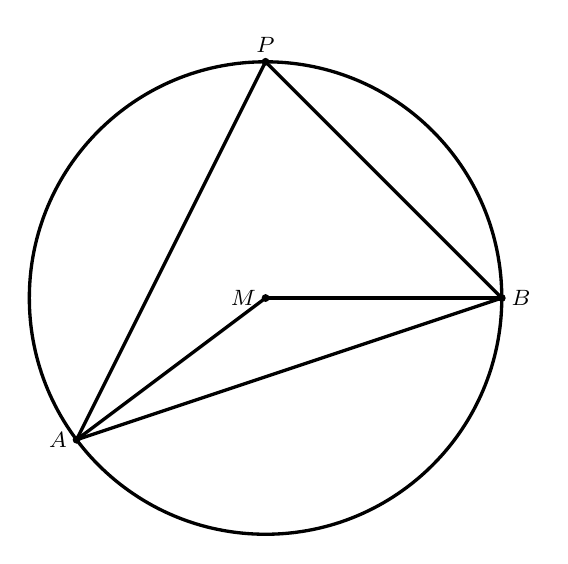
\begin{tikzpicture}[cross/.style={draw, cross out, minimum size=2*(#1-1pt), inner sep=0pt, outer sep=0pt}, x=1cm, y=1cm,
			>=latex,   %Voreinstellung für Pfeilspitzen
			font= \footnotesize, scale=0.6]
			\draw[black, very thick](-1,0) circle (5);
			\filldraw[black] (-1,0) circle (2pt) node[anchor=east]{$M$};
			\filldraw[black] (4,0) circle (2pt) node[anchor=west]{$B$};
			\filldraw[black] (-5,-3) circle (2pt) node[anchor=east]{$A$};
			\filldraw[black] (-1,5) circle (2pt) node[anchor=south]{$P$};
			\draw[black,very thick] (-5,-3) -- (4,0);
			\draw[black,very thick] (-5,-3) -- (-1,0);
			\draw[black,very thick] (-1,0) -- (4,0);
			\draw[black,very thick] (4,0) -- (-1,5);
			\draw[black,very thick] (-5,-3) -- (-1,5);
		\end{tikzpicture}
	\end{figure}
	\begin{aufgabe}
		Betrachte das folgende \href{https://www.geogebra.org/m/exmt29g4}{Geogebra-Applet}\footnotemark, in dem die beiden Punkte $A$ und $P$ verschoben werden können. Stelle basierend auf deinen Beobachtungen eine Behauptung auf, in der beide Winkel $\mu$ und $\phi$ vorkommen. \[\gap{1}\*\mu=\gap{1}\*\phi\]
		Nun möchten wir deine Behauptung auch beweisen.
		\begin{enumerate}
			\item Zeichne die Strecke $\overline{MP}$ ein.
			\item Stelle eine Formel für die Berechnung der Winkelsumme des Dreiecks $\triangle AMB$ und des Dreiecks $\triangle APB$ auf.
			\begin{align*}
				180^\circ &= \gap{5}\\
				180^\circ &= \gap{5}
			\end{align*}
			\item Da die linke Seite der beiden obigen Formel gleich sind, können die beiden rechten Seiten gleichgesetzt werden. \[\gap{5}=\gap{5}\] Forme die entstandene Gleichung nun soweit um, bis du deine Behauptung findest.
		\end{enumerate}
		\karos{4}
		Damit haben wir den Zentriwinkelsatz erfolgreich bewiesen.
	\end{aufgabe}
	\footnotetext{\url{https://www.geogebra.org/m/exmt29g4}}
	\begin{satz}[Zentriwinkelsatz]
		Der Zentriwinkel $\mu$ über einer Sehne $\overline{AB}$ ist genau doppelt so gross wie der zugehörige Peripheriewinkel $\phi$.
	\end{satz}
	Analog zum Zentriwinkelsatz können wir mithilfe des Geogebra-Applets auch noch den Peripheriewinkelsatz behaupten. Wir verzichten aber hier ausnahmsweise auf einen detailierten Beweis. Der Peripheriewinkelsatz besagt also folgendes:
	\begin{satz}[Peripheriewinkelsatz]
		Alle Peripheriewinkel $\phi$ über der gleichen Sehne $\overline{AB}$ sind gleich gross; i.e. Der Punkt $P$ kann frei verschoben werden, ohne dass sich der Winkel verändert.
	\end{satz}
	\begin{aufgabe}
		Löse die Aufgaben zum Peripherie- und Zentriwinkelsatz.
	\end{aufgabe}


\newpage
\section{Dreieckslehre}
	\begin{minipage}[t]{0.6\textwidth}
		Zur Erinnerung noch einmal die Standard-Bezeichnungen bei Dreiecken: \\
		Seiten werden mit dem gleichen (Klein-) Buchstaben wie der gegenüberliegende Eckpunkt beschriftet. Die Winkel mit dem entsprechenden griechischen Buchstaben des Eckpunktes.
	\end{minipage}
	\hfill
	\begin{minipage}[t]{0.375\textwidth}
		\vspace{-1cm}
		\centering
		\begin{tikzpicture}[cross/.style={draw, cross out, minimum size=2*(#1-1pt), inner sep=0pt, outer sep=0pt}, x=10mm, y=10mm,
			>=latex,   %Voreinstellung für Pfeilspitzen
			font= \footnotesize, scale=1]
			% Punkte definieren
			\coordinate (A) at (0,0.5);
			\coordinate (B) at (4,0);
			\coordinate (C) at (2.5,3);
			% Dreieck zeichnen und beschriften
			\draw[black, thick] (A) -- (B) -- (C) -- cycle;
			\draw[plotblue,fill=plotblue] (A) circle (2pt) node[left=4pt, above] {\normalsize$A$};
			\draw[plotblue,fill=plotblue] (B) circle (2pt) node[right] {\normalsize$B$};
			\draw[plotblue,fill=plotblue] (C) circle (2pt) node[above=2pt,right=2pt] {\normalsize$C$};
			\node at (3.5,1.5) {\normalsize$a$};
			\node at (1.1,2) {\normalsize$b$};
			\node at (2,0) {\normalsize$c$};
			\pic["\normalsize$\alpha$",draw,color=forestgreen,angle radius=8mm] {angle=B--A--C};
			\pic["\normalsize$\beta$",draw,color=forestgreen,angle radius=8mm] {angle=C--B--A};
			\pic["\normalsize$\gamma$",draw,color=forestgreen,angle radius=8mm] {angle=A--C--B};
 		\end{tikzpicture}
	\end{minipage}
	In diesem Kapitel wollen wir die Grundlagen im allgemeinen Dreieck repetieren und besondere Linien und Punkte im Dreieck sauber definieren. Damit wir im Anschluss in der Lage sind, uns präzise auszudrücken und spezielle Dreiecke, wie zum Beispiel gleichseitige, gleichschenklige oder rechtwicklige, untersuchen können.

\subsection{Die Höhen}
	\vspace{7pt}
	\begin{definition}
		Die \textbf{Höhe} eines Dreiecks ist die Senkrechte ausgehend von einem Eckpunkt auf die gegenüberliegende Seite (oder deren Verlängerung).
	\end{definition}
	Der Zusatz \flqq oder deren Verländerung\frqq\:ist vorallem bei stumpfwinkligen Dreiecken wichtig. Betrachte dazu die folgende Skizze:
	\begin{figure}[H]
		\centering
		\begin{tikzpicture}[cross/.style={draw, cross out, minimum size=2*(#1-1pt), inner sep=0pt, outer sep=0pt}, x=10mm, y=10mm,
			>=latex,   %Voreinstellung für Pfeilspitzen
			font= \footnotesize, scale=1]
			%Raster zeichnen
			\draw [color=gray!50]  [step=5mm] (0,0) grid (17,5.5);
			% Dreieck zeichnen
			\draw[black, thick] (2,5) -- (3,2.5) -- (6,2) -- (2,5);
			\draw[plotblue,fill=plotblue] (2,5) circle (2pt) node[left=4pt, above] {\normalsize$C$};
			\draw[plotblue,fill=plotblue] (3,2.5) circle (2pt) node[left=4pt, below] {\normalsize$A$};
			\draw[plotblue,fill=plotblue] (6,2) circle (2pt) node[right=8pt, below=-4pt] {\normalsize$B$};
		\end{tikzpicture}
	\end{figure}

\subsection{Winkelhalbierende}
	\vspace{7pt}
	\begin{aufgabe}
		Beschreibe in eigenen Worten, wie du eine Winkelhalbierende konstruieren würdest.\\[2pt]\karos{2.5}
	\end{aufgabe}
	In einem Dreieck können wir für jeden enthaltenen Winkel eine Winkelhalbierende konstruieren. Alle drei schneiden sich in einem einzigen Punkt.
	\begin{definition}
		Die \textbf{Winkelhalbierende} eines Dreiecks eine Halbgerade ausgehend von einem Eckpunkt, sodass der Winkel in diesem Punkt exakt halbiert wird.
	\end{definition}
	\begin{aufgabe}
		Betrachte das folgende \href{https://www.geogebra.org/m/jtrmgthn}{Geogebra-Applet}\footnotemark\:und beantworte die Frage: Was kannst du einen beliebigen Punkt auf einer Winkelhalbierenden aussagen, wenn du den Abstand des Punktes zu den beiden Schenkel vergleichst?\\[2pt]\karos{3.5}
	\end{aufgabe}
	\footnotetext{\url{https://www.geogebra.org/m/jtrmgthn}} Daraus kann folgende Konsequenz abgeleitet werden:
	\begin{satz}
		\begin{minipage}{0.475\textwidth}
			Der Schnittpunkt der drei Winkelhalbierenden von allen Winkeln eines Dreiecks ist der Mittelpunkt $M_I$ der \textbf{Inkreises}.
		\end{minipage}
		\hfill
		\begin{minipage}{0.5\textwidth}
			\centering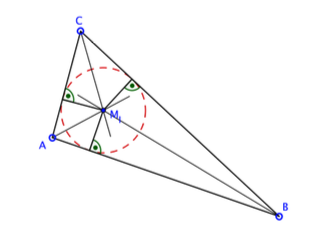
\includegraphics[height=4.5cm]{inkreis.png}
		\end{minipage}
	\end{satz}

\subsection{Mittelsenkrechte}
	\vspace{7pt}
	\begin{aufgabe}
		Beschreibe in eigenen Worten, welche Eigenschaft auf alle Punkte zutrifft, die auf der Mittelsenkrechte liegen.\\[2pt]\karos{2}
	\end{aufgabe}
	\begin{definition}
		Die \textbf{Mittelsenkrechte} in einem Dreieck steht senkrecht auf einer Seite und halbiert diese Seite in zwei exakt gleich lange Teilstrecken.
	\end{definition}
	\begin{minipage}[t]{0.475\textwidth}
		In einem Dreieck stellen wir fest, dass sich alle drei Mittelsenkrechten wiederum in einem einzigen Punkt schneiden. Dieser Punkt ist von allen drei Eckpunkten gleich weit entfernt und kann damit als Mittelpunkt eines weiteren Kreises benutzt werden.
	\end{minipage}
	\hfill
	\begin{minipage}[t]{0.5\textwidth}
		\vspace{-10pt}
		\centering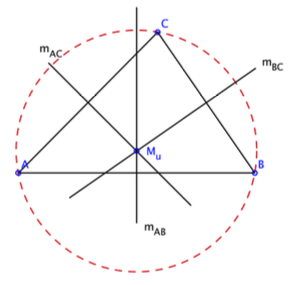
\includegraphics[scale=0.5]{umkreis.png}
	\end{minipage}
	\begin{satz}
		Der Schnittpunkt der drei Mittelsenkrechten zu allen Seiten eines Dreiecks ist der Mittelpunkt $M_U$ des Umkreis.
	\end{satz}

\subsection{Seitenhalbierende / Schwerlinie}
	\vspace{7pt}
	\begin{definition}
		Eine \textbf{Seitenhalbierende} oder \textbf{Schwerlinie} eines Dreiecks ist die Verbindungsstrecke von einem Eckpunkt zum gegenüberliegenden Seitenmittelpunkt. \\[2pt]
		Die Seitenhalbierenden werden nach der zugehörigen Seite resp. Punktes beschrieben: $ {s_a, s_b, s_c}$
	\end{definition}
	\begin{minipage}[t]{0.64\textwidth}
		So langsam bist Du sicher nicht mehr erstaunt, dass sich auch hier alle drei Linien \textbf{in einem Punkt schneiden}.	Eine wichtige Eigenschaft erkennt man vermutlich, wenn man die folgenden Streckenlängen misst und vergleicht:
		\begin{table}[H]
			\begin{tabular}{llllll}
				$\overline{AS}$ & $=$ & \gap{2} cm \hspace{10mm} & $\overline{SM_{BC}}$ & $=$ & \gap{2} cm  \\[4mm]
				$\overline{BS}$ & $=$ & \gap{2} cm \hspace{10mm} & $\overline{SM_{AC}}$ & $=$ & \gap{2} cm  \\[4mm]
				$\overline{CS}$ & $=$ & \gap{2} cm \hspace{10mm} & $\overline{SM_{AB}}$ & $=$ & \gap{2} cm  \\[2mm]
			\end{tabular}
		\end{table}
	\end{minipage}
	\hfill
	\begin{minipage}[t]{0.34\textwidth}
		\vspace{0pt}
		\centering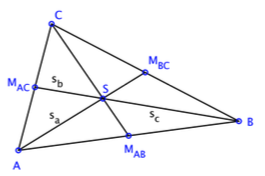
\includegraphics[scale=0.6]{seitenhalbierende.png}
	\end{minipage}
	Ein Eckpunkt ist vom Schwerpunkt $S$ immer \textbf{doppelt so weit} entfernt wie der zugehörige Seitenmittelpunkt. \\[1mm]
	\begin{satz}
		Der Schwerpunkt $S$ teilt die Seitenhalbierende im Verhältnis $2\: : \:1$.
	\end{satz}
	\begin{aufgabe}
		Löse die Aufgaben zu den speziellen Linien und Punkte im Dreieck.
	\end{aufgabe}


\newpage
\subsection*{History}
\begin{table}[H]
	\centering
	\begin{tabular}{|p{13mm}|p{20mm}|p{30mm}|p{70mm}|}\hline
		%\multicolumn{4}{|l|}{History}\\\hline
		Version & Datum & Person & Bemerkung \\\hline
		$1.0$ & 14.09.2024 & Jonas Guler & Kapitel erstellt \\\hline
		$1.1$ & 01.10.2026 & Jonas Guler & Abschnitt zu den speziellen Linien und Punkte im Dreieck ergänzt. \\\hline
		$1.2$ & ToDo & Jonas Guler & Aufgaben zusammensuchen \\\hline
	\end{tabular}
\end{table}


\end{document}